\documentclass{elsarticle}

\journal{Annals of Nuclear Energy}
%%%% packages and definitions (optional)
\newcommand{\Cyclus}{\textsc{Cyclus}\xspace}%
\newcommand{\Cycamore}{\textsc{Cycamore}\xspace}

\usepackage{tabularx}
\usepackage[acronym,toc]{glossaries}
\include{acros}
\makeglossaries
\usepackage{xspace}

\usepackage{caption}
\newcolumntype{b}{X}
\newcolumntype{s}{>{\hsize=.5\hsize}X}
\newcolumntype{m}{>{\hsize=.75\hsize}X}



\usepackage{tikz}
\usetikzlibrary{shapes.geometric,arrows}
\tikzstyle{process} = [rectangle, rounded corners, minimum width=3cm, minimum height=1cm,text centered, draw=black, fill=blue!30]
\tikzstyle{object} = [ellipse, rounded corners, minimum width=3cm, minimum height=1cm,text centered, draw=black, fill=green!30]
\tikzstyle{arrow} = [thick,->,>=stealth]
\usetikzlibrary{positioning, arrows, decorations, shapes }%


\begin{document}
\begin{frontmatter}

\title{Modeling High-fidelity Molten Salt Reactor in a Large-Scale Fuel Cycle Simulation}
\author{Jin Whan Bae$^{1}$, Andrei Rykhlevskii$^{1}$, Benjamin R. Betzler$^{2}$, Joshua L. Peterson-Droogh$^{2}$, Kathryn Huff$^{1}$}
\address{$^{1}$Dept. of Nuclear, Plasma, and Radiological Engineering, University of Illinois at Urbana-Champaign, Urbana, IL \\ $^{2}$Oak Ridge National Laboratory, Oak Ridge, TN }

\begin{abstract}
We developed a method to model \glspl{MSR} in large-scale fuel cycle
simulations by roughly coupling two reactor physics code SERPENT
and SCALE suite of codes. We used Saltproc, an in-house developed
python wrapper to simulate \gls{MSR} behavior in SERPENT. SCALE
has a in-code method of modeling constant addition and removal
of material by editing the Bateman equation. We postprocess the
results from each code to a standardized HDF5 format with
the stream isotopics flow history. We simulated the \gls{MSR}
behavior in \Cyclus, an agent-based simulator, using a \Cyclus archetype
that interprets the HDF5 database that mimics the material flow in and
out of the reactor. This method provides a rapid and high-fidelity
way of modeling \glspl{MSR} in a large-scale fuel cycle simulation.
\end{abstract}

\end{frontmatter}

	

\section{Introduction}

\glspls{MSR} are difficult to model in fuel cycle
simulations due to their continuous reprocessing, where
there is a continuous flow of materials in and out of
the reactors. Many modules have been developed to model
continuous reprocessing in an \gls{MSR}. 



\subsection{\Cyclus}

\Cyclus is an agent-based fuel cycle simulation framework 
\cite{huff_fundamental_2016}, which means 
that each reactor, reprocessing plant, and fuel fabrication plant is modeled as an agent.
A \Cyclus simulation contains prototypes, which are fuel cycle facilities with
pre-defined parameters, that are deployed in the simulation as \texttt{facility} agents.
Encapsulating the \texttt{facility} agents are the \texttt{institution} and \texttt{region}.
A \texttt{region} agent holds a set of \texttt{institution}s.
An \texttt{institution} agent can deploy or decommission \texttt{facility} agents.
The \texttt{institution} agent is part of a \texttt{region} agent,
which can contain multiple \texttt{institution} agents. Several versions of \texttt{Institution}
and \texttt{region} exist, varying in complexity and functions \cite{huff_extensions_2014}.
 \texttt{DeployInst} is used as the institution archetype for this work, where the institution
deploys agents at user-defined timesteps.

At each timestep (one month),
agents make requests for materials or bid to supply them and exchange
with one another. A market-like mechanism called the dynamic resource exchange
\cite{gidden_agent-based_2015} governs the exchanges.
Each material resource has a quantity, composition, name, and a unique identifier
for output analysis. The timestep execution in \Cyclus follows 
\texttt{Build, Tick,} \gls{DRE}, \texttt{Tock, and Decommission}, as illustrated in
figure \ref{fig:time}. The \texttt{Tick}, and \texttt{Tock} phases are for
each agent to perform actions, such as transmutation, separation, or generation
of materials before and after the market exchange phase.

\begin{figure}[h]
\centering
\scalebox{0.7}{
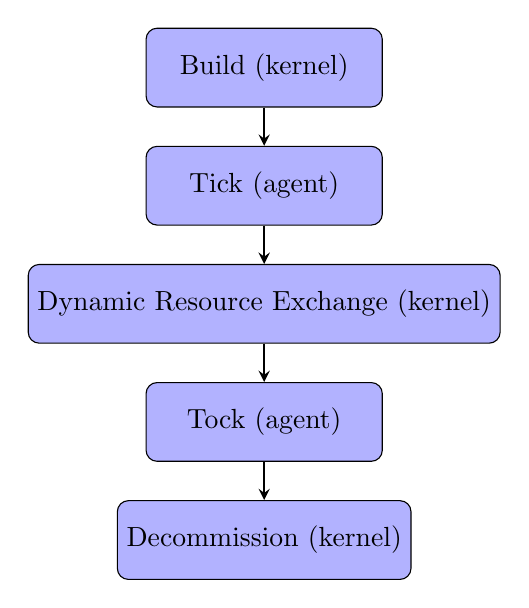
\begin{tikzpicture}[node distance=1.5cm]
\node (Build) [process] {Build (kernel)};
\node (Tick) [process, below of=Build] {Tick (agent)};
\node (DRE) [process, below of=Tick]{Dynamic Resource Exchange (kernel) };
\node (Tock) [process, below of=DRE]{Tock (agent)};
\node (Decom) [process, below of=Tock] {Decommission (kernel)};

\draw [arrow] (Build) -- (Tick); 
\draw [arrow] (Tick) -- (DRE);
\draw [arrow] (DRE) -- (Tock);
\draw [arrow] (Tock) -- (Decom);
\end{tikzpicture}
}
\caption{\Cyclus timestep execution steps.}
\label{fig:time}
\end{figure}

The modularity of \Cyclus allows a low barrier of
entry for developers, since developers can create an
archetype (e.g. Reactor module, Reprocessing module)
without extensive knowledge of the \Cyclus framework.

\subsection{Saltproc}
Saltproc is an external python driver developed to
model batch-wise reprocessing in \glss{MSR}. The code
repeatedly runs SERPENT, performs material operations (e.g. reprocessing,
inflow of fertile material), and saves all material flow
and k-eff values in a HDF5 database. 

\section{Methodology}

[Development of full-core SERPENT MODELS AND OTHER THINGS ANDREI DID]

Then we perform continuous reprocessing analysis on the developed
SERPENT models using Saltproc. The reprocessing scheme is as follows:

[Reprocessing scheme - if different for reactor, mention it]

Note that some reactors have two regions, a driver and a blanket region.
Saltproc is capable of reprocessing from one region and inputting
the separated flow to the other region. For example, plutonium is bred
in the blanket region of a MCSFR, which is separated and input into
the driver region. 

Saltproc also has a reactivity control model, which controls the reactivity
by controlling the amount of fissile material put into the core. At
every depletion step, the k-eff value is checked and modifications
to the fissile stream is made accordingly.


We run the Saltproc for the entire fuel cycle of each \gls{MSR}. For example,
if a \gls{MSR} design asks for a salt-flush (complete unloading of core)
every ten years, the fuel cycle time of the \gls{MSR} would be ten years.
This way, the entire material flow history of the \gls{MSR} is captured
in the Saltproc output database.

The output database is then loaded into the Cyclus module.
The module reads the timestep of the database and the timestep of Cyclus,
and outputs the corresponding waste and surplus fissile stream every timestep.
The module also requests the corresponding amount of fertile material
that the reactor needs from the market. In short, the purpose of the module is to
mimic the interaction of a \gls{MSR} with the market, while producing
power. The module's interaction with the framework is illustrated in
figure \ref{fig:msr_int}.


\begin{figure}[htbp!]
    \begin{center}
        \includegraphics[scale=0.5]{./images/msr_flowchart.png}
    \end{center}
        \caption{Interaction of Cyclus \gls{MSR} module with the Cyclus framework (Market)}
    \label{fig:msr_int}
\end{figure}

\section{Results}

[Results showing MSR behavior]

[Material flow from and out of MSR]

[Mass deployment of MSR]

[Reprocessing of MSR fuel]

[Two different MSRs in Synergy with Each other]

[LWR reprocessing to fuel MSRs]
\section{Discussion}

Leveraging the modularity and agent-based structure of \Cyclus,
we can mimic the fuel cycle impact of \glspl{MSR} using a database
generated from a high-fidelity reactor physics calculation.
This database-approach outsources the computationally heavy
calculations outside the fuel cycle simulation, and allows
for quick, high-resolution implementation of complex systems
in the nuclear fuel cycle.
\input{acks}

\bibliographystyle{elsarticle-num}
\bibliography{bibliography}


\end{document}
